\documentclass{article}
\usepackage[utf8]{inputenc}
\usepackage[T1]{fontenc}
\usepackage{lmodern}
\usepackage{amsmath, amssymb}
\usepackage{graphicx}
\usepackage{hyperref}
\usepackage{geometry}
\geometry{margin=1in}

\usepackage{pgfplots}
\pgfplotsset{compat=1.17}


\title{Comparing the Efficiency of Machine Learning and Deep Learning Models in Source Code Authorship Attribution}
\author{Richard Čerňanský}
\date{\today}

\begin{document}
\maketitle

\begin{abstract}
\end{abstract}

\section{Introduction}
Introduction


\section{Methods}
Methods

\section{Results}


\begin{table}[h!]
    \centering
    {\scriptsize
    \begin{tabular}{lcccc}
    \hline
    \multicolumn{5}{c}{\textbf{Models' Author Attribution Accuracy for Different Author Set Sizes}} \\
    \hline
    \textbf{Model} & \multicolumn{4}{c}{\textbf{Author Set Size}} \\
    \cline{2-5}
                  & 110  & 27  & 11 & 3 \\ 
    \hline
    Random Forests (TF--IDFs w/o comments) & 66.24\%\;|\;$3.63\,\mathrm{min}$ & 70.60\%\;|\;$0.23\,\mathrm{min}$ & 80.56\%\;|\;$0.08\,\mathrm{min}$ & 85.84\%\;|\;$0.05\,\mathrm{min}$ \\
    BERT (source code w/o comments)        & 72.47\%\;|\;$70.33\,\mathrm{min}$ & 82.72\%\;|\;$32.49\,\mathrm{min}$ & 89.84\%\;|\;$9.34\,\mathrm{min}$  & 90.70\%\;|\;$1.82\,\mathrm{min}$ \\
    BERT (AST pre\_order traversal)        & 24.07\%\;|\;$73.53\,\mathrm{min}$ & 35.66\%\;|\;$30.00\,\mathrm{min}$ & 40.62\%\;|\;$5.69\,\mathrm{min}$  & 83.72\%\;|\;$1.22\,\mathrm{min}$ \\
    AttentionNN (AST paths)              & --- & --- & --- & --- \\
    \hline
    \end{tabular}
    }
    \caption{Comparison of models across author attribution accuracy and training time for different author set sizes.}
    \label{tab:comparison}
\end{table}


\begin{figure}[h!]
\centering
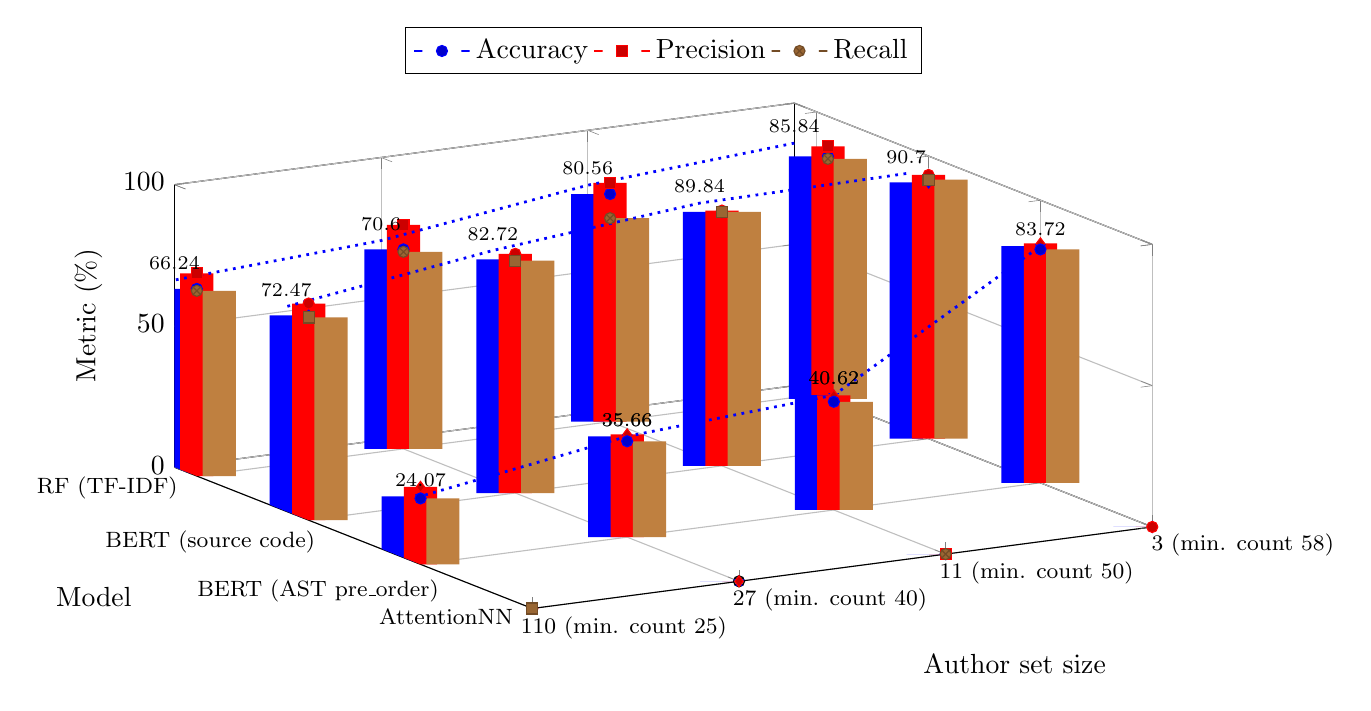
\begin{tikzpicture}
\begin{axis}[
    view={60}{30},            % 3D viewing angles (azimuth, elevation)
    z buffer=sort,            % Ensures correct front-to-back rendering
    xlabel={Model},
    xlabel style={
        xshift = -40pt,
        yshift=40pt,
        align=center          % optional alignment
    },
    ylabel={Author set size},
    ylabel style={
        xshift = 25pt,
        yshift=20pt,
        align=center          % optional alignment
    },
    zlabel={Metric (\%)},
    width=14cm,
    height=8cm,
    xtick={1,2,3,4},
    xticklabels={RF (TF-IDF), BERT (source code), BERT (AST pre\_order), AttentionNN},
    xticklabel style={
        font=\footnotesize,    % or \footnotesize, \tiny, etc.
        xshift = -20pt,
        yshift=10pt,
        align=center          % optional alignment
    },
    ytick={4,3,2,1}, % Reversed ytick values
    yticklabels={3 (min. count 58), 11 (min. count 50), 27 (min. count 40), 110 (min. count 25)}, % Corresponding reversed labels
    yticklabel style={
        font=\footnotesize,    % or \footnotesize, \tiny, etc.
        xshift = 25pt,
        yshift=5pt,
        align=center          % optional alignment
    },
    zmin=0, zmax=100,
    grid=major,
    legend style={
        at={(0.5,1.15)},
        anchor=north,
        legend columns=3
    }
]

%%%%%%%%%%%%%%%%%%%%%%%%%%%%%%%%%%%%%%%%%%%%%%%%%%%%%%%%%%%%%%
% MODEL 1: RF (x = 1)
%%%%%%%%%%%%%%%%%%%%%%%%%%%%%%%%%%%%%%%%%%%%%%%%%%%%%%%%%%%%%%

\addplot3+[ybar, bar width=12pt, fill=blue, draw=none, bar shift=-0.2]
    coordinates {(1.1,4,85.84) (1,3,80.56) (1,2,70.60) (1,1,66.24)}; % Coordinates are adjusted to match the reversed ytick
\addplot3+[ybar, bar width=12pt, fill=red, draw=none, bar shift=0]
    coordinates {(1.1,4,89.36) (1,3,84.56) (1,2,79.27) (1,1,71.73)}; % Coordinates are adjusted to match the reversed ytick
\addplot3+[ybar, bar width=12pt, fill=brown, draw=none, bar shift=+0.2]
    coordinates {(1.1,4,84.96) (1,3,72.03) (1,2,69.73) (1,1,65.55)}; % Coordinates are adjusted to match the reversed ytick

    %dotted line
\addplot3+[
    mark=none,
    blue,
    dotted,
    line width=1pt,
    nodes near coords,
    every node near coord/.append style={
        mark=none,
        fill=none,
        draw=none,
        text=black,
        font=\scriptsize,
        yshift=0pt
    }
] coordinates {
    (0.8,4,85.84) (0.8,3,80.56) (0.8,2,70.60) (0.8,1,66.24) % Coordinates are adjusted to match the reversed ytick
};

%%%%%%%%%%%%%%%%%%%%%%%%%%%%%%%%%%%%%%%%%%%%%%%%%%%%%%%%%%%%%%
% MODEL 2: BERT-SOURCE (x = 2)
%%%%%%%%%%%%%%%%%%%%%%%%%%%%%%%%%%%%%%%%%%%%%%%%%%%%%%%%%%%%%%

\addplot3+[ybar, bar width=12pt, fill=blue, draw=none, bar shift=-0.2]
    coordinates {(2,4,90.70) (2,3,89.84) (2,2,82.72) (2,1,72.47)}; % Coordinates are adjusted to match the reversed ytick
\addplot3+[ybar, bar width=12pt, fill=red, draw=none, bar shift=0]
    coordinates {(2,4,93.33) (2,3,90.33) (2,2,84.66) (2,1,76.69)}; % Coordinates are adjusted to match the reversed ytick
\addplot3+[ybar, bar width=12pt, fill=brown, draw=none, bar shift=+0.2]
    coordinates {(2,4,91.67) (2,3,89.92) (2,2,82.25) (2,1,71.76)}; % Coordinates are adjusted to match the reversed ytick

\addplot3+[
    mark=none,
    blue,
    dotted,
    line width=1pt,
    nodes near coords,
    every node near coord/.append style={
        mark=none,
        fill=none,
        draw=none,
        text=black,
        font=\scriptsize,
        yshift=0pt
    }
] coordinates {
    (1.8,4,90.70) (1.8,3,89.84) (1.8,2,82.72) (1.8,1,72.47) % Coordinates are adjusted to match the reversed ytick
};

%%%%%%%%%%%%%%%%%%%%%%%%%%%%%%%%%%%%%%%%%%%%%%%%%%%%%%%%%%%%%%
% MODEL 3: BERT-AST (x = 3)
%%%%%%%%%%%%%%%%%%%%%%%%%%%%%%%%%%%%%%%%%%%%%%%%%%%%%%%%%%%%%%

\addplot3+[ybar, bar width=12pt, fill=blue, draw=none, bar shift=-0.2]
    coordinates {(3,4,83.72) (3,3,40.62) (3,2,35.66) (3,1,24.07)}; % Coordinates are adjusted to match the reversed ytick
\addplot3+[ybar, bar width=12pt, fill=red, draw=none, bar shift=0]
    coordinates {(3,4,84.72) (3,3,40.53) (3,2,36.41) (3,1,27.40)}; % Coordinates are adjusted to match the reversed ytick
\addplot3+[ybar, bar width=12pt, fill=brown, draw=none, bar shift=+0.2]
    coordinates {(3,4,82.58) (3,3,38.30) (3,2,33.93) (3,1,23.33)}; % Coordinates are adjusted to match the reversed ytick
\foreach \yA/\zA/\yB/\zB in {
    4/83.72/3/40.62,
    3/40.62/2/35.66,
    2/35.66/1/24.07
} {
    \addplot3+[
        mark=none,
        blue,
        dotted,
        line width=1pt,
        nodes near coords,
        every node near coord/.append style={
            mark=none,
            fill=none,
            draw=none,
            text=black,
            font=\scriptsize,
            yshift=0pt
        }
    ] coordinates {
        (3,\yA,\zA) (3,\yB,\zB)
    };
}

%%%%%%%%%%%%%%%%%%%%%%%%%%%%%%%%%%%%%%%%%%%%%%%%%%%%%%%%%%%%%%
% MODEL 4: ATTENTION-NN (x = 4) - Data missing => set to 0
%%%%%%%%%%%%%%%%%%%%%%%%%%%%%%%%%%%%%%%%%%%%%%%%%%%%%%%%%%%%%%
\foreach \yy in {1,2,3,4} {
    \addplot3+[ybar, bar width=12pt, fill=blue, draw=none, bar shift=-0.2] coordinates {(4,\yy,0)};
    \addplot3+[ybar, bar width=12pt, fill=red, draw=none, bar shift=0] coordinates {(4,\yy,0)};
    \addplot3+[ybar, bar width=12pt, fill=brown, draw=none, bar shift=+0.2] coordinates {(4,\yy,0)};
}

%%%%%%%%%%%%%%%%%%%%%%%%%%%%%%%%%%%%%%%%%%%%%%%%%%%%%%%%%%%%%%
% LEGEND
%%%%%%%%%%%%%%%%%%%%%%%%%%%%%%%%%%%%%%%%%%%%%%%%%%%%%%%%%%%%%%
\addplot3[
    ybar, 
    fill=blue, 
    draw=none, 
    bar width=12pt, 
    legend image code/.code={
        \draw[fill=blue] (0cm,-0.1cm) rectangle (0.6cm,0.1cm);
    }
] coordinates {(0,0,-9999)};
\addlegendentry{Accuracy}

\addplot3[
    ybar, 
    fill=red, 
    draw=none, 
    bar width=12pt, 
    legend image code/.code={
        \draw[fill=red] (0cm,-0.1cm) rectangle (0.6cm,0.1cm);
    }
] coordinates {(0,0,-9999)};
\addlegendentry{Precision}

\addplot3[ % Recall
    ybar, 
    fill=brown, 
    draw=none, 
    bar width=12pt, 
    legend image code/.code={
        \draw[brown, mark=x] plot coordinates {(0cm,0cm)}; 
    }
] coordinates {(0,0,-9999)};
\addlegendentry{Recall} 

\end{axis}
\end{tikzpicture}
\caption{Bar chart comparing Accuracy (with accuracy values labeled), Precision, and Recall across models and author set sizes with minimum function count per author. }
\label{fig:3d-bars-legend-brown}
\end{figure}

\section{Discussion}
Here we discuss the implications of our results. 


\section{Conclusion}
We conclude that this document compiles successfully. If you can read all sections, view the figure, and see the mathematical expressions, your LaTeX environment is correctly set up.

\end{document}
